\chapter{Analiza dziedziny problemu}
W dzisiejszych czasach, przed firmami archeologicznymi stoi nie małe wyzwanie, polegające na przeprowadzaniu badań archeologicznych na coraz większych powierzchniowo obszarach. Badanie archeologiczne przedinwestycyjne (w których specjalizuje się firma "JN-Profil" - docelowy użytkownik oprogramowania stworzonego w ramach niniejszej pracy) polegają na przeprowadzeniu badań terenowych oraz stworzeniu dokumentacji podsumowującej rezultaty tych badań.

Dokumentacja archeologiczna zawiera w sobie dużą liczbę dokumentów, z których conajmniej część opiera się na tych samych danych, których proces przetwarzania można, a nawet powinno sie zautomatyzować. Do tej pory, tworzenie dokumentacji sprowadzało się do mozolnego kopiowania danych z jednego miejsca do drugiego, jednak dzięki współcześnie dostępnym technologiom informatycznym istnieje możliwość zautomatyzowania i przyspieszenia tego procesu - co w szerszej perspektywie prowadzi do zmniejszenia kosztów przeprowadzania badań archeologicznych.

\section{Wymgagania biznesowe}
Przed systemem do prowadzenia ewidencji badań archeologicznych jest stawiany szereg wymagań, których spełnienie jest warunkiem poprawnego funkcjonowania oraz zadowolenia użytkowników. Część z nich jest wspólna dla wszystkich systemów informatycznych, natomiast reszta jest związana z charakterem pracy archeologa.

Aby system nadawał się do profesjonalnego użytku konieczne jest, aby efekty pracy były zapisane w pamięci trwałej. Konieczne jest także, aby możliwe było równoległe korzystanie wielu użytkowników, z dodatkowym zastrzerzeniem, że równoległe sesje użytkowników mogą pracować na tych samych danych i system powinien mimo to gwarantować spójność danych.

Specyficzną cechą pracy archeologa jest konieczność wyjazdów i prowadzenia badań archeologicznych w różnych miejscach. System wspierający prowadzenie ewidencji badań archeologicznych powinien umożliwiać tworzenie dokumentacji z różnych miejsc i urządzeń. 
\newpage
\section{Model dziedziny problemu}
W systemie wspierającym działalność firmy archeologicznej, powinno się wyróżnić 6 najważniejszych elementów:
\begin{itemize}
\item Zabytki Masowe\\
\item Zabytki Wydzielone\\
\item Obiekty Archeologiczne\\
\item Zdjęcia\\
\item Rysunki\\
\item Ary
\end{itemize}

Wszystkie powyższe obiekty są produktem przeprowadzanego badania archeologicznego, dlatego są bytami, które mają sens tylko w konkretnym kontekscie biznesowym (czyli opracowaniu). Wszystkie inne informacje wprowadzone do systemu są uniwersalne dla badań archeologicznych, dlatego są dostępne i edytowalne niezależnie od opracowania.
\newpage
\begin{figure} [H]
    \begin{center}
	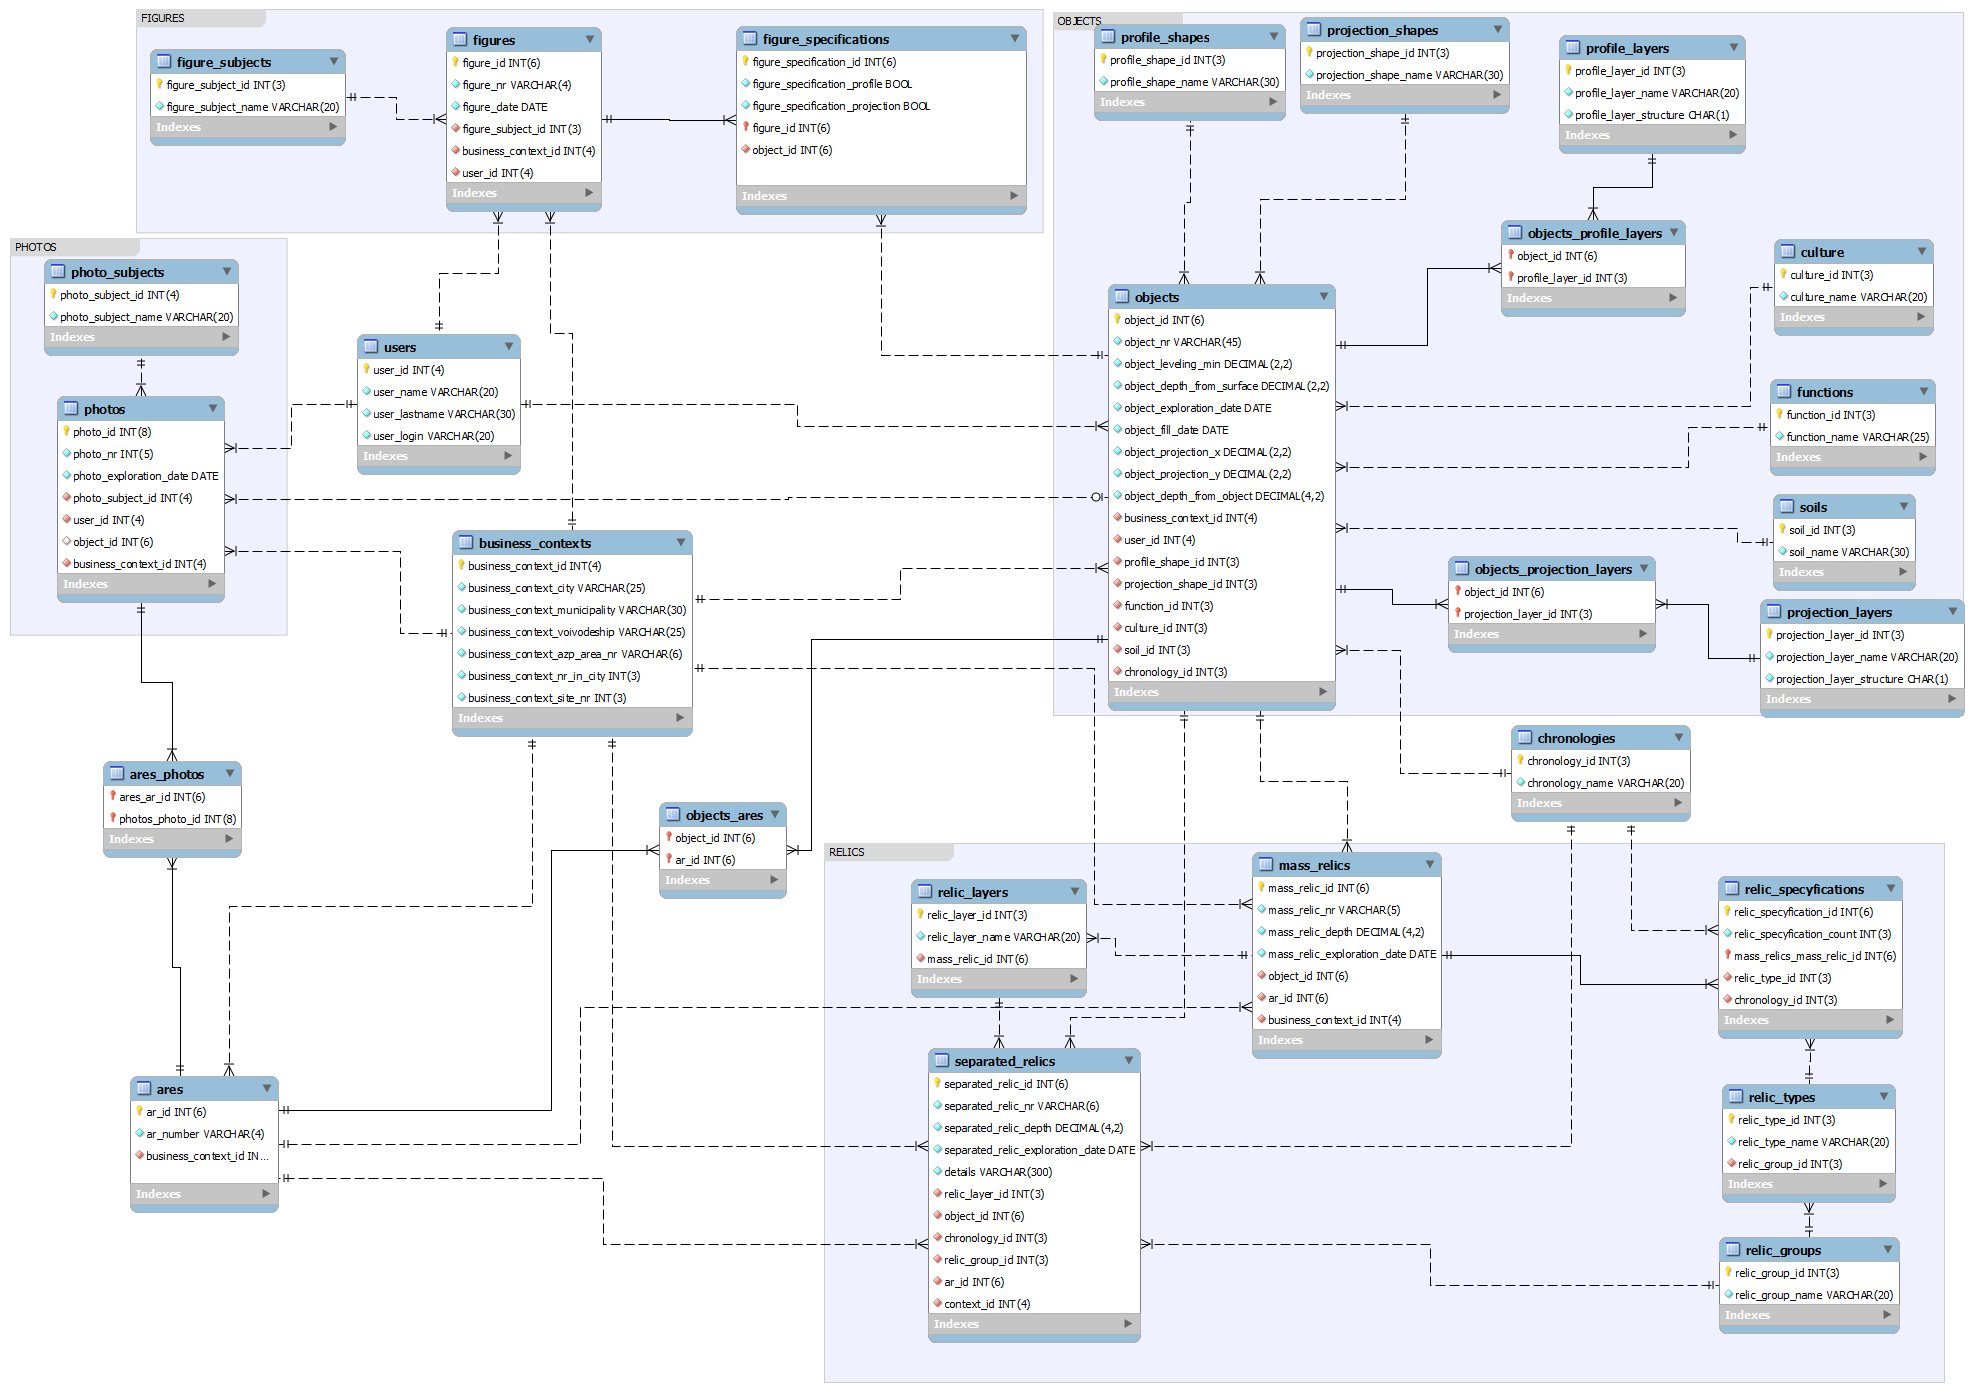
\includegraphics[angle=90, scale=.26]{img/db.png}
	\caption{Model dziedziny}
	\label{modelDziedziny}
    \end{center}
\end{figure}

\section{Model przypadków użycia}
Zadaniem systemu wspierającego tworzenie dokumentacji archeologicznej powinno być umożliwienie wprowadzenia danych w łatwy i przejrzysty sposób oraz szybkie generowanie raportów, będących składnikami dokumentacji archeologicznej.

\begin{figure} [H]
    \begin{center}
	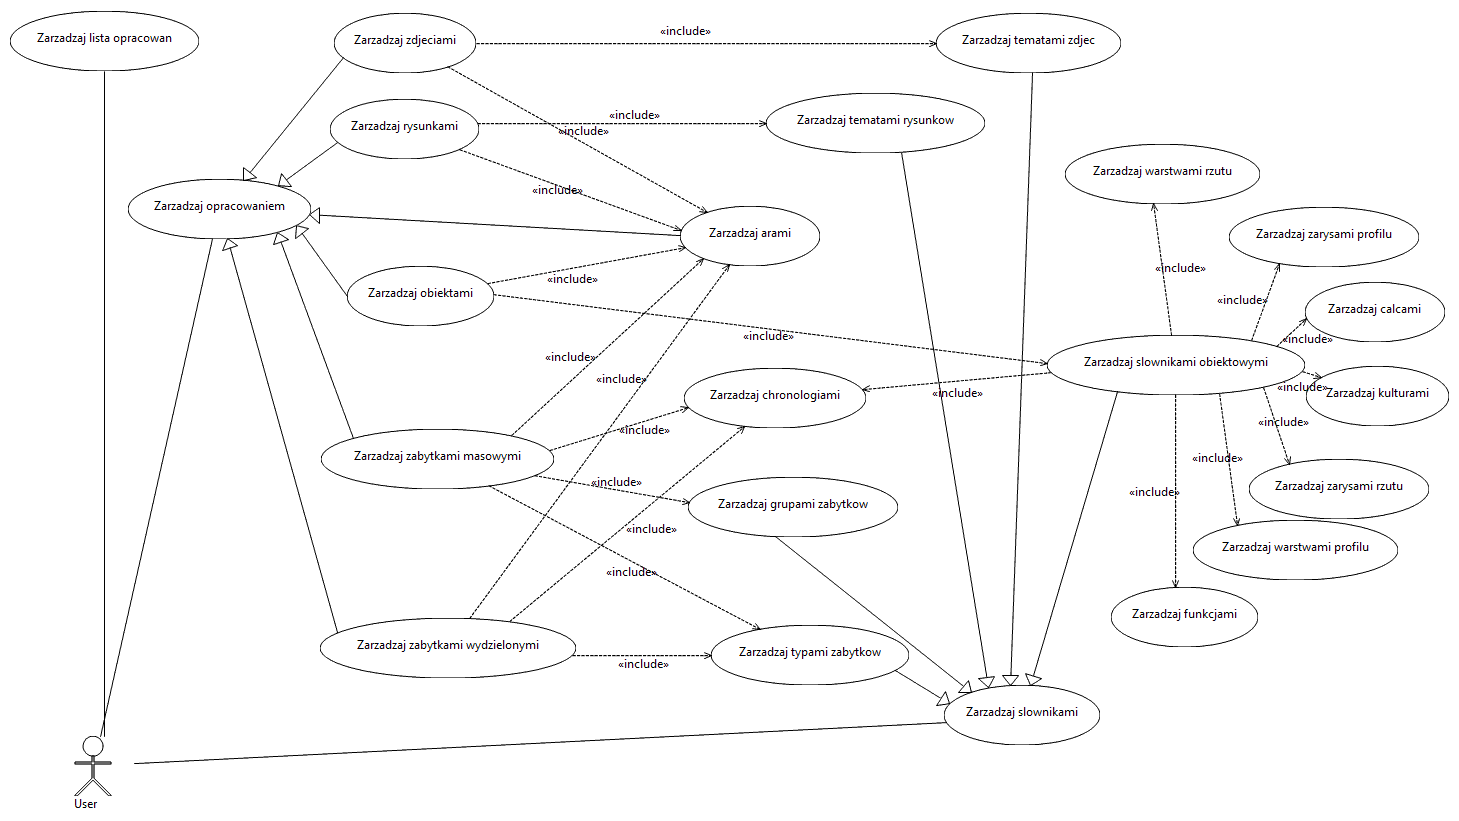
\includegraphics[angle=90, scale=.35]{img/useCasesData.png}
	\caption{Diagram przypadków użycia}
	\label{useCasesDiag}
    \end{center}
\end{figure}

Dodatkową cechą systemu będącego produktem niniejszej pracy jest to, że możliwa jest edycja słowników służących do wypełniania danych z poziomu okna edycji obiektu wypełnianego.
\newpage
\section{Struktura aplikacji}

Standardowy ekran aplikacji wygląda jak na poniższym rysunku.

\begin{figure} [H]
    \begin{center}
	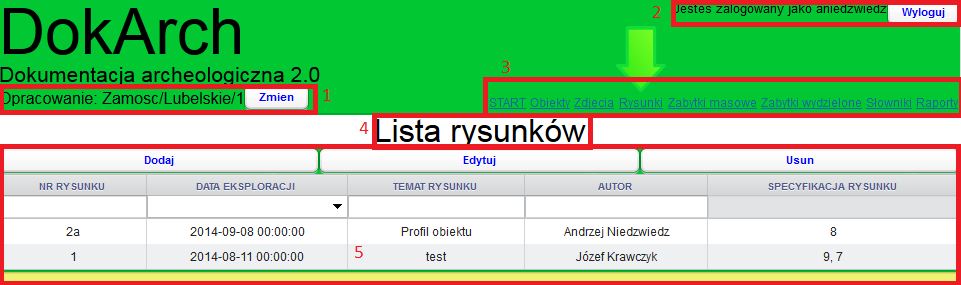
\includegraphics[scale=.6]{img/strona.png}
	\caption{Przykładowa podstrona systemu}
	\label{stronaPrzyklad}
    \end{center}
\end{figure}

Na załączonym obrazku widać, że strona aplikacji składa się z:
\begin{itemize}
\item górnej belki zawierającej w sobie informacje o bieżącym opracowaniu (1 na rysunku), informacje o zalogowanym użytkowniku (2) oraz menu (3)
\item belki tytułowej (4)
\item głównej treści strony (5) 
\end{itemize}

Powyższy rysunek demonstruje także przykładowy widok listujący wprowadzone dane (w tym przypadku rysunki). Dzięki addonowi FilterTable, możliwe jest filtrowanie widocznych elementów po ich zawartości w konkretnych polach. Standardowa funkcjonalność Vaadina pozwala także sortować wiersze wg wartości w kolumnie - w tym celu wystarczy kliknąć nagłówek kolumny.

\begin{figure} [H]
    \begin{center}
	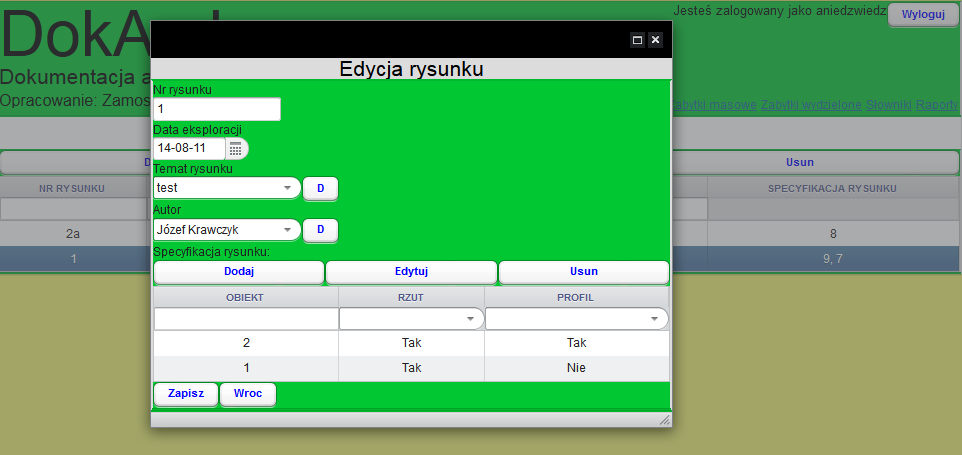
\includegraphics[scale=.6]{img/edycja.png}
	\caption{Przykładowa edycja obiektu dokumentacyjnego}
	\label{edycjaPrzyklad}
    \end{center}
\end{figure}

\newpage
Rysunek znajdujący się nad tym tekstem demonstruje ekran edycji wiersza (w tym przypadku wiersz odzwierciedla ewidencjonowany rysunek). 

\begin{figure} [H]
    \begin{center}
	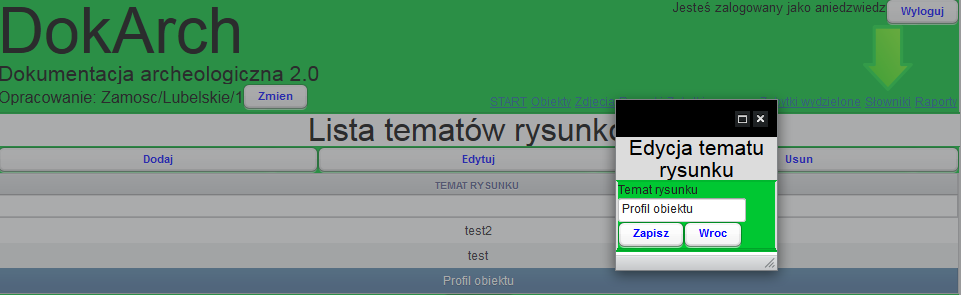
\includegraphics[scale=.6]{img/edycjaSlownika.png}
	\caption{Przykładowa edycja słownika}
	\label{edycjaSlownika}
    \end{center}
\end{figure}

Rysunek powyżej przedstawia standardowy sposób edycji słownika (wybranie w menu w górnej belce "Słowniki" a następnie wybranie słownika "Tematy rysunków"). Jest to jeden ze sposobów modyfikacji wartości słownika.

\begin{figure} [H]
    \begin{center}
	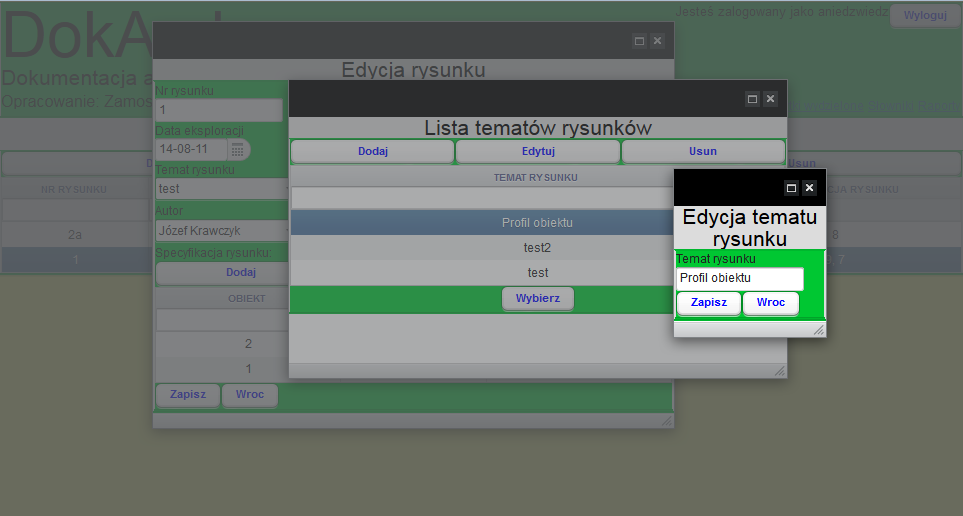
\includegraphics[scale=.6]{img/edycjaSlownikaWLocie.png}
	\caption{Przykładowa edycja słownika w trakcie edycji obiektu używającego go}
	\label{edycjaSlownikaWLocie}
    \end{center}
\end{figure}

Powyżej został przedstawiony ekran modyfikacji słownika w ``locie", czyli w trakcie edycji wiersza, który zawiera wartość ze słownika. Możliwe jest dynamiczne wprowadzanie wartości bez konieczności zamykania okna edycji.

% ex: set tabstop=4 shiftwidth=4 softtabstop=4 noexpandtab fileformat=unix filetype=tex spelllang=pl,en spell: